%!TEX root = ./template-skripsi.tex
%-------------------------------------------------------------------------------
%                            BAB III
%               			PEMBAHASAN
%-------------------------------------------------------------------------------

\chapter{METODOLOGI PENELITIAN}

\begin{spacing}{1.5}

% \section{Keterhubungan Penelitian}

% \begin{figure}[H]
% 	\centering
% 	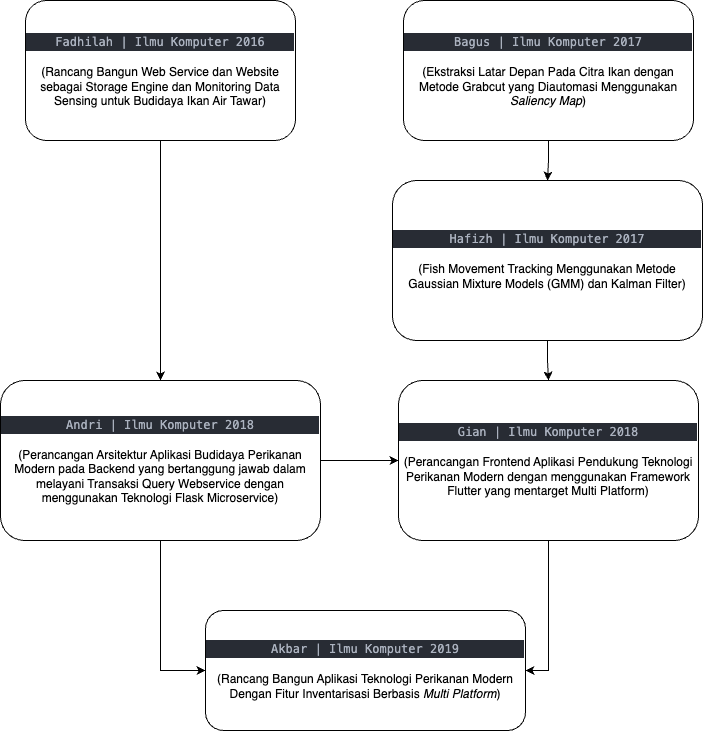
\includegraphics[width=0.7\textwidth]{gambar/research_tree.png}
% 	\caption{Diagram Alur Penelitian \textit{Aquaculture}}
% \end{figure}

% Pada diagram diatas, dapat dilihat urutan arah dari topik penelitian Aquaculture. Penelitian pertama kali dimulai oleh \citep{fadhil2021} dengan mengembangkan sebuah \textit{web service} serta \textit{website} yang berfungsi sebagai \textit{storage engine} dan \textit{monitoring data sensing} untuk digunakan pada budidaya perikanan air tawar sebagai media penyimpanan data-data sensing dari sensor yang dikirimkan ke sistem serta memonitoringnya dalam bentuk table dan grafik \textit{real-time} serta penelitian yang dilakukan oleh \citep{bagus2022} dengan tujuan untuk membangun sistem deteksi objek pada citra ikan dengan metode GrabCut yang telah diautomasi menggunakan \textit{saliency map}.

% Penelitian \citep{bagus2022} kemudian dilanjutkan oleh \citep{hafiz2021} yaitu merancang dan membangun sebuah sistem yang dapat melakukan pelacakan pergerakan ikan dengan menggunakan metode GMM dan Kalman Filter. Sementara penelitian \citep{fadhil2021} belum diterapkan pada aplikasi riset \textit{Aquaculture} dalam waktu dekat sehingga penelitian yang dibuat oleh \citep{andri2022} dilakukan dengan membuat \textit{web service} juga yang bertujuan untuk melayani transaksi \textit{query} berupa monitoring budidaya perikanan yang dibarengi dengan penelitian \citep{gian2022} pada bagian perancangan \textit{frontend} sebagai pendukung pada aplikasi yang dikembangkan.

% Dalam penelitian yang sudah berjalan ini, penulis mengembangkan penelitian yang dilakukan oleh \citep{andri2022} dan \citep{gian2022} dengan membuat fitur baru yaitu manajemen inventaris yang dapat menentukan harga dasar dari produk hasil perikanan.

\section{Inventaris Budidaya Perikanan}

Inventaris pada budidaya perikanan mencakup keperluan yang digunakan selama menjalankan masa budidaya, inventaris tersebut dapat dikategorikan menjadi inventaris pakan, inventaris suplemen, inventaris listrik, inventaris benih, dan inventaris aset.

Masing-masing inventaris memiliki detail tersendiri, detail tersebut dapat dilihat dari contoh tabel inventaris berikut.

% \hfill \break
% \hfill \break
% \hfill \break
% \hfill \break
% \hfill \break

\begin{enumerate}
	\item Inventaris Pakan
	
	\begin{figure}[H]
		\centering
		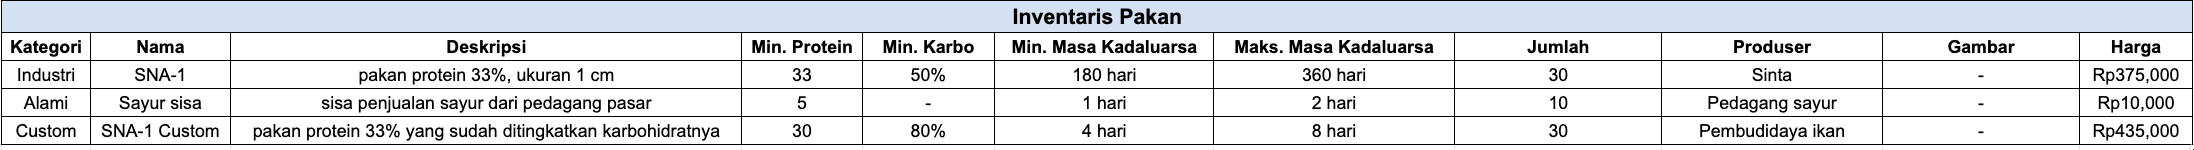
\includegraphics[width=1\textwidth]{gambar/tabel_inventaris_pakan.png}
		\caption{Contoh Tabel Data Inventaris Pakan}
	\end{figure}	

	Pada tabel ini, terdapat beberapa detail dari inventaris pakan antara lain kategori pakan, merk pakan, deskripsi pakan, protein dan karbo pakan, masa kadaluarsa pakan, jumlah pakan, produser pakan, serta harga pakan.

	\hfill \break
	\hfill \break
	\hfill \break
	\hfill \break


	\item Inventaris Suplemen
	
	\begin{figure}[H]
		\centering
		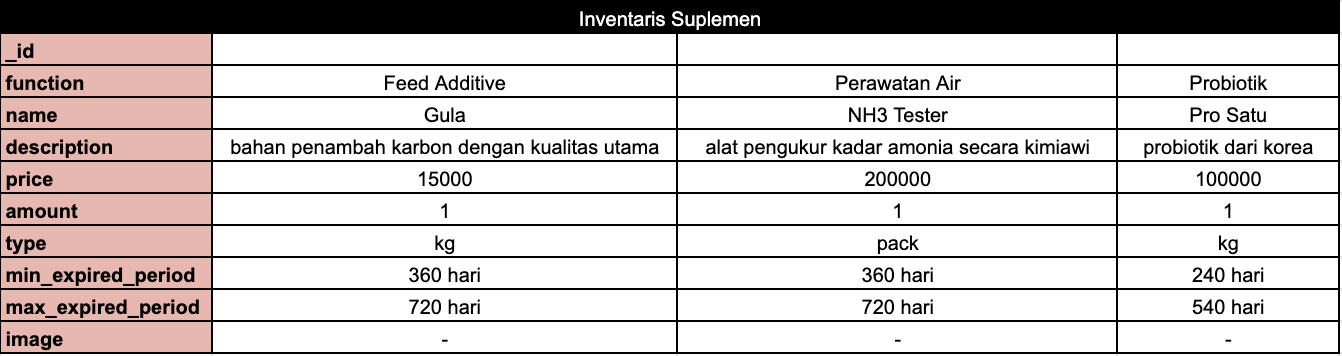
\includegraphics[width=1\textwidth]{gambar/tabel_inventaris_suplemen.png}
		\caption{Contoh Tabel Data Inventaris Suplemen}
	\end{figure}

	Pada tabel ini, tedapat beberapa detail dari inventaris suplemen antara lain fungsi suplemen, nama suplemen, deskripsi suplemen, harga suplemen, jumlah suplemen, tipe satuan suplemen, serta masa kadaluarsa suplemen.

	\item Inventaris Listrik
	
	\begin{figure}[H]
		\centering
		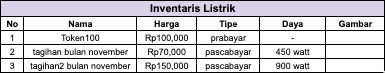
\includegraphics[width=1\textwidth]{gambar/tabel_inventaris_listrik.png}
		\caption{Contoh Tabel Data Inventaris Listrik}
	\end{figure}	

	Pada tabel ini, terdapat beberapa detail dari inventaris listrik antara lain nama, harga, tipe, daya, nomor token serta bulan bayar dari listrik.

	\hfill \break
	\hfill \break
	\hfill \break
	\hfill \break

	\item Inventaris Benih
	
	\begin{figure}[H]
		\centering
		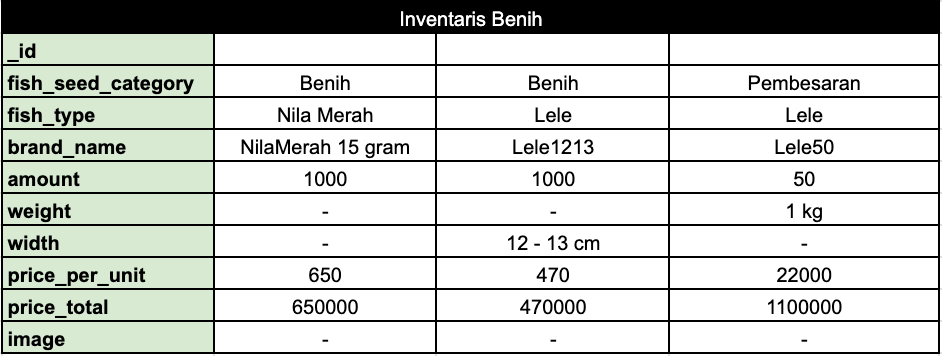
\includegraphics[width=1\textwidth]{gambar/tabel_inventaris_benih.png}
		\caption{Contoh Tabel Data Inventaris Benih}
	\end{figure}	

	Pada tabel ini, terdapat beberapa detail dari inventaris benih antara lain kategori benih, tipe ikan, nama ikan, jumlah benih, berat benih, ukuran benih, harga benih per ekor serta harga benih total.

	\item Inventaris Aset
	
	\begin{figure}[H]
		\centering
		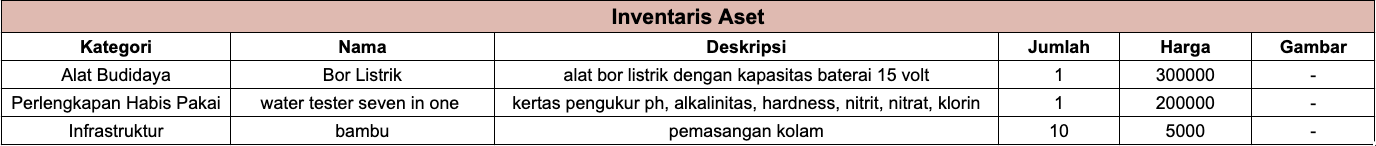
\includegraphics[width=1\textwidth]{gambar/tabel_inventaris_aset.png}
		\caption{Contoh Tabel Data Inventaris Aset}
	\end{figure}	

	Pada tabel ini, terdapat beberapa detail dari inventaris aset antara lain kategori aset, nama aset, deskripsi aset, jumlah serta harga aset per unit.

\end{enumerate}

\section{Metode Penentuan Harga Dasar}

Dalam penentuan harga dasar, penulis melakukan diskusi dengan Dinas Pertanian dan Perikanan Bogor. Berikut merupakan gambaran pada saat diskusi berlangsung.


\begin{figure}[H]
	\hspace{.05\linewidth}
	\minipage{0.32\textwidth}
		
\includegraphics[width=1.5\linewidth]{gambar/disk1.jpg}
		\caption{Diskusi dengan Dinas Pertanian dan Perikanan Bogor}
	\endminipage
	\hspace{.18\linewidth}
	\minipage{0.32\textwidth}%
		
\includegraphics[width=1.5\linewidth]{gambar/disk2.jpg}
		\caption{Diskusi dengan Dinas Pertanian dan Perikanan Bogor}
	\endminipage
	\hspace{.05\linewidth}
\end{figure}


Dari diskusi tersebut, didapatkan hasil berupa rumus penentuan harga sebagai berikut.

% Ketika musim budidaya sudah selesai dan kolam sudah bisa untuk dipanen, maka harga ikan sementara yang bisa digunakan dapat dihitung dengan rumus-rumus berikut.

% Dalam beberapa skenario, harga jual ditentukan oleh pedagang kepada pembudidaya. Harga ini dijamin lebih kecil dibanding harga retail, karena pedagang akan mengambil keuntungan dari itu. Jika dimisalkan T adalah harga jual minimum agar pembudidaya tidak rugi, $W_{feed}$ sebagai total pakan yang diberikan dan P adalah harga satuan pakan. Maka hubungan dari variabel-variabel tersebut adalah sebagai berikut.
% \begin{equation}
%     \begin{split}
% 		T
% 		&= W_{feed} \times P
%     \end{split}
% \end{equation}

% Rumus ini didasari oleh konversi antara kilogram pakan menjadi pertambahan berat sebagian besar bervariasi tergantung pada kasus tertentu. Terlepas dari itu ditentukan oleh semakin tinggi asupan protein, maka semakin rendah tingkat konversinya. Jika konversi ini dikaitkan sebagai Food Conversion Ratio  (FCR) yang dimana $W_{fish}$ sebagai total berat dari semua ikan yang dipanen.
% \begin{equation}
%     \begin{split}
% 		FCR
% 		&= W_{feed } \div W_{fish}
%     \end{split}
% \end{equation}

% Oleh karena itu, pembudidaya harus mencatat berapa banyak kilogram pakan yang diberikan sampai musim panen dari tiap kolam untuk menemukan nilai FCR-nya. Dalam masalah yang lebih kompleks, jika pakan memungkinkan datang dari berbagai sumber yang berhubungan dengan variasi asupan protein, FCR tidak dapat digunakan untuk menentukan hubungan antara jumlah pakan dan pertambahan berat.  Maka dari itu, sangat direkomendasikan untuk pembudidaya agar menggunakan satu sumber asupan protein tiap musim panen. Karena FCR sudah diketahui, selama musim panen berikutnya pembudidaya bisa memperkirakan berapa banyak pakan yang dibutuhkan untuk membuat ikan agar tumbuh sampai ukuran yang ditargetkan.
% \begin{equation}
%     \begin{split}
% 		W_{fish}
% 		&= W_{feed} \div FCR
%     \end{split}
% \end{equation}

% Dengan itu bisa digunakan dalam mencari total jumlah pakan yang dibutuhkan untuk membuat ikan agar tumbuh sampai ukuran yang ditargetkan. 
% \begin{equation}
%     \begin{split}
% 		W_{feed}
% 		&= W_{fish} \times FCR
%     \end{split}
% \end{equation}

% Jika persamaan 4 dikembangkan dengan memasukkan dua variabel yaitu $W_i$ sebagai berat ikan dan n sebagai jumlah ikan, maka persamaan akan menjadi seperti berikut.
% \begin{equation}
%     \begin{split}
% 		W_{fish}
% 		&= \sum_{i=1}^n \times W_i
%     \end{split}
% \end{equation}

% Namun, menggunakan persamaan 5 akan mematikan tujuan dari persamaan 4, karena jika ingin menghitung pemakaian pakan diharuskan untuk menilai masing-masing ikan secara individu yang dimana itu tidak praktis. Jika menggunakan variabel $W_{af}$ sebagai rata-rata dari berat ikan, maka persamaan akan menjadi sebagai berikut.
% \begin{equation}
%     \begin{split}
% 		W_{af}
% 		&= \frac{\sum_{i=1}^n \times W_i}{n}
%     \end{split}
% \end{equation}

% Sekarang dapat dengan mudah mencari perkiraan konsumsi pakan untuk musim panen berikutnya dengan persamaan,
% \begin{equation}
%     \begin{split}
% 		W_{feed}
% 		&= W_{af} \times n \times FCR
%     \end{split}
% \end{equation}


% Jika persamaan 1 diupdate sehingga dapat ditemukan harga sesuai dengan persamaan,
% \begin{equation}
%     \begin{split}
% 		T_{unit}
% 		&= \frac{T}{n}
%     \end{split}
% \end{equation}

% Persamaan itu juga merujuk pada jumlah perdagangan dalam kilogram, oleh karena itu
% \begin{equation}
%     \begin{split}
% 		k
% 		&= \frac{1kg}{W_{af}}
%     \end{split}
% \end{equation}

% \begin{equation}
%     \begin{split}
% 		T_k
% 		&= T_{unit} \times k
%     \end{split}
% \end{equation}

% Sebagai contoh, dimisalkan mata uang yang digunakan adalah koin lalu FCR bernilai 1.5, ukuran target panen adalah 4 ikan per kilogram, di kolam terdapat 1000 ikan, dan harga pakan mencapai 10 koin.

% Dari data tersebut, dapat diketahui $W_{af}$ = 1/4 kg, n = 1000. Karena itu, $W_{feed}$ bernilai 375 kg yang harus dipersiapkan. Selanjutnya, pembudidaya tidak bisa menjual semua hasil panen ikan seharga dibawah T = 3750 koin atau dibawah 15 koin per kilogram.

% Persamaan 1 sampai 10 memungkinan jika FCR konstan dengan treatment yang sama dan asupan protein yang sama. Seperti yang sudah dilakukan diawal, pembudidaya harus mengandalkan satu sumber protein tetapi untuk mempertahankan hal ini sulit dilakukan. Karena itu, PER (Protein Efficiency Ratio) diketahui untuk menentukan rasio massa tubuh yang diperoleh dengan gram protein yang dikonsumsi. Disini variabel $P_{feed}$ mendefinisikan asupan gram protein.
% \begin{equation}
%     \begin{split}
% 		PER
% 		&= \frac{W_{fish}}{P_{feed}}
%     \end{split}
% \end{equation}

% Pada formula tersebut, menggantikan $W_{feed}$ pada persamaan 2 dengan $P_{feed}$ akan memberikan bentuk variabel yang sama namun struktur variabel yang terbalik. Hal ini juga memberikan kemungkinan untuk mencampur beberapa sumber protein yang berbeda dengan formula berikut.
% \begin{equation}
%     \begin{split}
% 		PER
% 		&= \frac{W_{fish}}{P^1_{feed} + P^2_{feed} + \dots + P^k_{feed}}
%     \end{split}
% \end{equation}

% \begin{equation}
%     \begin{split}
% 		PER
% 		&= \frac{W_{fish}}{\sum_{i=1}^k \times P^i_{feed}}
%     \end{split}
% \end{equation}

% Variabel k mengartikan jumlah dari sumber protein yang berbeda. Hal ini juga dapat dilakukan pada FCR dan T sebagai berikut.
% \begin{equation}
%     \begin{split}
% 		FCR
% 		&= \frac{\sum_{i=1}^k \times W^k_{feed}}{W_{fish}}
%     \end{split}
% \end{equation}
% \begin{equation}
%     \begin{split}
% 		T
% 		&= \sum_{i=1}^k \times W^k_{feed} \times P
%     \end{split}
% \end{equation}

% Pada persamaan 15, hanya memodelkan harga jual minimum barang perikanan agar terhindar dari kerugian. Karena itu, untuk mendapatkan keuntungan diperlukan model yang baru. Disini variabel $T_p$ melambangkan dagangan yang memberikan keuntungan dan $F_g$ sebagai pendapatan pembudidaya.
% \begin{equation}
%     \begin{split}
% 		T_p
% 		&= T + F_g
%     \end{split}
% \end{equation}

% $F_g$ merepresentasikan berapa banyak jam kerja yang dilakukan pembudidaya untuk membudidayakan ikan. Hal ini dapat dijelaskan lebih rinci dalam
% \begin{equation}
%     \begin{split}
% 		F_g
% 		&= D \times S
%     \end{split}
% \end{equation}

% Dimana D mengartikan berapa banyak hari pembudidaya bekerja sampai musim panen dan S mengartikan upah yang mewakili pendapatan pekerjaan. Dalam berbudidaya, merupakan hal umum bagi pembudidaya ikan untuk menghabiskan waktu seharian penuh untuk mengembangkan dan memantau kolam, karena itu representasi hari lebih ideal. Sebab itu, pembudidaya yang lebih banyak menghabiskan waktunya sampai musim panen tiba harus mendapatkan pendapatan yang sesuai.

% Persamaan 15 berlaku jika budidaya ikan membudidayakan ikan tradisional secara tradisional. Dalam sistem intensif aquaculture khususnya BFT, dibutuhkan variabel yang mewakili biaya tambahan yang dikeluarkan untuk penggunaan teknologi. Variabel ${C_i}$ merepresentasikan masing-masing biaya tambahan yang dikeluarkan dalam BFT untuk keseluruhan musim kawin.
% \begin{equation}
%     \begin{split}
% 		T
% 		&= \sum_{i=1}^k \times W^k_{feed} \times P + \sum_{i=1}^l \times C_i
%     \end{split}
% \end{equation}

% Variabel $C_i$ dapat dijabarkan sebagai berikut.

% \begin{itemize}
% 	\item $C_1$ = Bahan baku (termasuk pakan dan suplemen)
% 	\item $C_2$ = Listrik (dihitung dalam per kolam)
% 	\item $C_3$ = Tenaga kerja (dihitung 3-5 jam / orang serta dibagi dengan jumlah kolam)
% 	\item $C_4$ = Benih ikan
% \end{itemize}

\begin{itemize}
	% \item Harga Dasar Produk
	
	% \begin{equation}
	% 	\begin{split}
	% 		T
	% 		&= \frac{C_p + C_q + C_r + \frac{C_l}{n}}{N}
	% 	\end{split}
	% \end{equation}

	% Dari formula ini, dapat dihasilkan harga dasar produk perikanan per ekornya. Ini dihitung berdasarkan detail pemakaian saat budidaya berlangsung seperti pakan, benih, obat-obatan dan perawatan air, serta pemakaian listrik per kolam.

	% \begin{itemize}
	% 	\item T = Harga jual minimum ikan
	% 	\item $C_p$ = Harga total benih selama musim berjalan
	% 	\item $C_q$ = Harga total pakan selama musim berjalan
	% 	\item $C_r$ = Harga total suplemen selama musim berjalan
	% 	\item $C_l$ = Harga tagihan listrik
	% 	\item n = Jumlah kolam
	% 	\item N = Jumlah ikan yang hidup
	% \end{itemize}	

	\item Harga Jual Minimum Produk
	
	\begin{equation}
		\begin{split}
			T
			&= \frac{C_p + C_q + C_r + \frac{C_l}{nA} + \frac{C_a}{60 * nB}}{N}
		\end{split}
	\end{equation}

	Dari formula ini, dapat dihasilkan harga jual minimum produk perikanan per ekornya. Perhitungan ini didapat dari hasil diskusi antara penulis dengan klien yang merupakan pembudidaya ikan.

	Detail atribut dari rumus dapat dilihat sebagai berikut.

\end{itemize}

\begin{itemize}
	\item T = Harga jual minimum ikan
	\item $C_p$ = Harga total pemakaian benih selama musim berjalan
	\item $C_q$ = Harga total pemakaian pakan selama musim berjalan
	\item $C_r$ = Harga total pemakaian suplemen selama musim berjalan
	\item $C_l$ = Harga tagihan listrik per bulannya
	\item $C_a$ = Harga total penggunaan aset
	\item nA = Jumlah kolam aktif
	\item nB = Jumlah semua kolam
	\item N = Jumlah ikan yang hidup pada kolam selama musim berjalan
\end{itemize}



Harga dari perhitungan tersebut dapat digunakan oleh pembudidaya untuk menjadi harga dasar dalam penjualannya. Tentunya harga tersebut merupakan harga panen atau produksi berdasarkan pengeluaran selama musim berjalan dan pembudidaya tidak wajib menggunakan harga tersebut dalam transaksi.

% \section{Depresiasi Aset Bahan Organik}

% Dalam menyimpan bahan baku pada inventaris, bahan baku tersebut akan mengalami penurunan karena bahan baku mempunyai masa kadaluarsa. Maka dari itu, dapat dimisalkan jika per bulan bahan baku tersebut mengalami penurunan kualitas sebesar 25\% dari harga belinya, maka dalam 4 bulan bahan baku tersebut akan kadaluarsa dan sudah tidak lagi berharga. Namun, skala penurunan tersebut bervariasi tergantung pada jenis bahan baku yang digunakan. Variabel $W_p$ mewakili harga dari bahan baku yang digunakan dan variabel $\alpha$ mewakili skala depresiasi per bulan dari bahan baku yang digunakan. Formula depresiasi dapat dibuat menjadi persamaan berikut.

% \begin{equation}
%     \begin{split}
% 		W_psesudah
% 		&= W_psebelum\times(1 - \alpha)
%     \end{split}
% \end{equation}

% \begin{itemize}
% 	\item $W_p$ = Harga dari bahan baku yang digunakan
% 	\item $\alpha$ = skala depresiasi per bulan dari bahan baku yang digunakan
% \end{itemize}

% Formula depresiasi tersebut dapat berlaku jika masa minimum kadaluarsa bahan organik telah terpenuhi, sebagai contoh dapat dilihat pada kasus berikut.

% Jika sayur sisa untuk pakan ikan memiliki masa minimum kadaluarsa yaitu 1 hari dengan harga Rp10.000,00/10 kg, maka formula depresiasi akan berlaku setelah 1 hari pemasukkan pakan tersebut dengan hitungan sebagai berikut ($\alpha$ = 0.5).

% \begin{enumerate}
% 	\item $W_psebelum$ = Rp10.000
% 	\item $\alpha$ = 0.5
% \end{enumerate}

% Maka, dapat dihitung dengan formula depresiasi sebagai berikut.

% \begin{equation*}
% 	\begin{aligned}
% 	W_psesudah &= W_psebelum\times(1 - \alpha)\\
% 	W_psesudah &= 10000\times(1 - 0.5)\\
% 	W_psesudah &= 5000
% 	\end{aligned}
% \end{equation*}

% Akan didapatkan $W_psesudah$ sebesar Rp5.000 yang akan terus berkurang sampai masa maksimum kadaluarsa dengan formula perhitungan yang sama. Masa maksimum ini dapat ditentukan oleh pengguna atau bisa secara otomatis ditentukan oleh sistem dengan perhitungan dua kali masa minimum kadaluarsa.

% Sebagai contoh, jika masa minimum kadaluarsa sayur sisa untuk pakan ikan yaitu 1 hari maka untuk masa maksimum kadaluarsa sayur sisa tersebut adalah 2 hari. Setelah 2 hari, maka nilai dari bahan tersebut ($Wp$) akan menjadi 0 (tidak bernilai) sehingga tidak termasuk dalam perhitungan harga dasar dan harga jual.

\section{Tahapan Penelitian}

\begin{figure}[H]
	\centering
	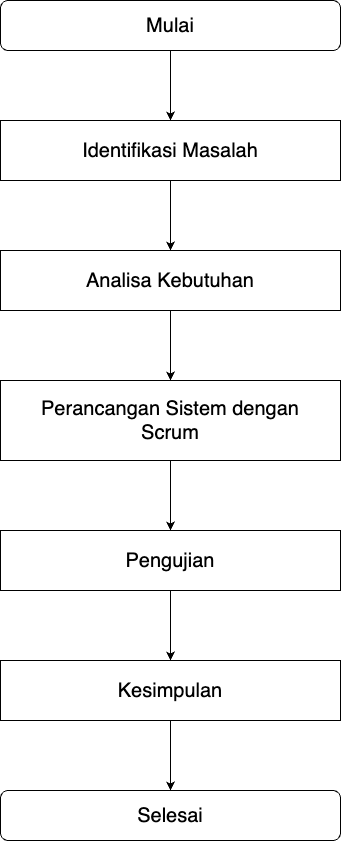
\includegraphics[width=0.35\textwidth]{gambar/tahapan_penelitian.png}
	\caption{Alur Tahapan Penelitian}
\end{figure}

Desain penelitian adalah alur yang dijalankan selama masa pengembangan aplikasi. Pada \textbf{Gambar 3.7}, terdapat desain penelitian yang digunakan dalam pembuatan aplikasi ini dengan metode Scrum.

% \section{Analisa Arsitektur Fitur}

% Pada penelitian aplikasi yang sudah dikembangkan sebelumnya, terdapat use case yang menjelaskan konsep dari aplikasi yang ada pada gambar dibawah ini.

% \begin{figure}[H]
% 	\centering
% 	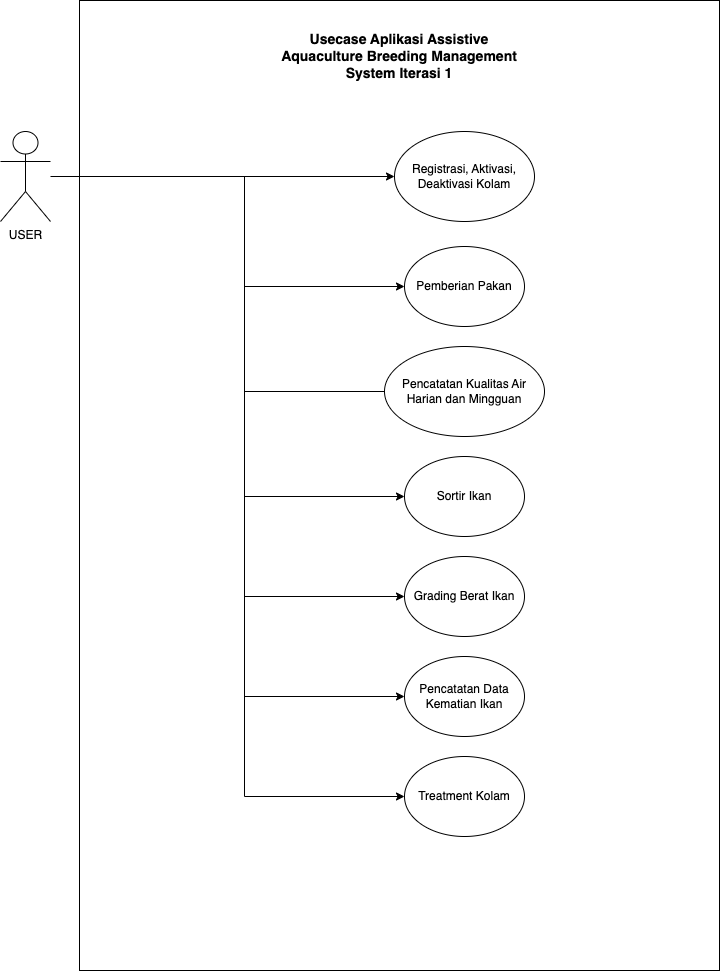
\includegraphics[width=0.8\textwidth]{gambar/usecase_iterasi_1.png}
% 	\caption{Use Case Fitur Aplikasi pada Iterasi 1}
% \end{figure}

% Dari diagram use case tersebut, terdapat dua jenis pengguna yaitu user dan admin. User dan admin memiliki fitur yang sama dalam aplikasi tersebut, yang membedakan antara user dan admin adalah skala prioritas dari aplikasi. Sisi admin memungkinkan pengguna dapat mengatur lebih banyak fitur yang ada pada aplikasi dan mendapatkan akses untuk mengatur user non-admin. Fitur yang disediakan aplikasi dijelaskan sebagai berikut.

% \begin{enumerate}
% 	\item \textbf{Registrasi, Aktivasi, Deaktivasi Kolam} = Fitur ini digunakan untuk mendaftarkan kolam yang akan dijadikan tempat budidaya ikan, kemudian fitur aktivasi dan deaktivasi kolam digunakan untuk mengontrol kolam yang sedang berjalan.
% 	\item \textbf{Pemberian Pakan} = Fitur ini digunakan untuk mencatat data pakan yang diberikan pada kolam ikan di budidaya yang sedang berlangsung.
% 	\item \textbf{Pencatatan Kualitas Air Harian dan Mingguan} = Fitur ini digunakan untuk mencatat kualitas air dari kolam di budidaya yang sedang berjalan dengan rentang waktu harian dan mingguan.
% 	\item \textbf{Sortir Ikan} = Fitur ini digunakan untuk mengatur perpindahan ikan ke kolam lain.
% 	\item \textbf{Grading Berat Ikan} = Fitur ini digunakan untuk mengatur ekosistem ikan berdasarkan berat agar mendapatkan keseragaman ukuran ikan dan meningkatkan efektivitas pemberikan pakan kepada ikan.
% 	\item \textbf{Pencatatan Data Kematian Ikan} = Fitur ini digunakan untuk mencatat angka kematian ikan jika terdapat ikan yang mati ketika budidaya sedang berjalan.
% 	\item \textbf{Treatment Kolam} = Fitur ini digunakan untuk melakukan pengaturan terhadap kolam ikan pada budidaya yang sedang berjalan.
% \end{enumerate}
\section{Analisa Kebutuhan}

Pada pengembangan aplikasi lanjutan ini, fitur yang ditambahkan adalah fitur manajemen inventaris serta fitur pembukuan. Fitur pencatatan inventaris merupakan fitur yang akan ada pada aplikasi yang berguna untuk para pembudidaya ikan mencatat semua hal yang berhubungan dengan budidaya perikanannya. Hal-hal yang dapat dicatat oleh pembudidaya pada fitur ini seperti bahan baku (termasuk pakan dan suplemen), penggunaan listrik, benih, serta aset yang digunakan selama masa budidaya dilakukan.

Selain mencatat inventaris pada musim budidaya, fitur pencatatan inventaris ini juga dapat menentukan rekomendasi harga jual dari ikan yang dipanen oleh pembudidaya ikan berdasarkan perhitungan dari pengeluaran biaya selama musim budidaya berjalan. Beberapa fitur yang sudah ada di penelitian sebelumnya juga harus diperbarui dengan adanya manajemen inventaris ini seperti panen, pemberian pakan, sortir ikan, serta treatment kolam.

Kemudian untuk fitur pembukuan berguna untuk pembudidaya ikan melihat riwayat musim budidaya yang sudah mereka jalankan. Terdapat beberapa rincian yang ditampilkan seperti biaya pengeluaran sampai berapa total ikan yang terpanen pada musim budidaya tersebut.

Fitur-fitur tersebut dapat dibuat menjadi \textit{use case} pada \textbf{Gambar 3.8}. Pada \textit{use case} tersebut, font warna hitam merupakan fitur yang sudah ada pada penelitian sebelumnya yang tidak berubah dan font warna cokelat merupakan fitur sebelumnya yang akan diperbarui pada penelitian ini. Sementara itu, untuk font warna hijau merupakan fitur baru yang akan tersedia pada aplikasi dan dikembangkan pada penelitian ini.

\begin{figure}[H]
	\centering
	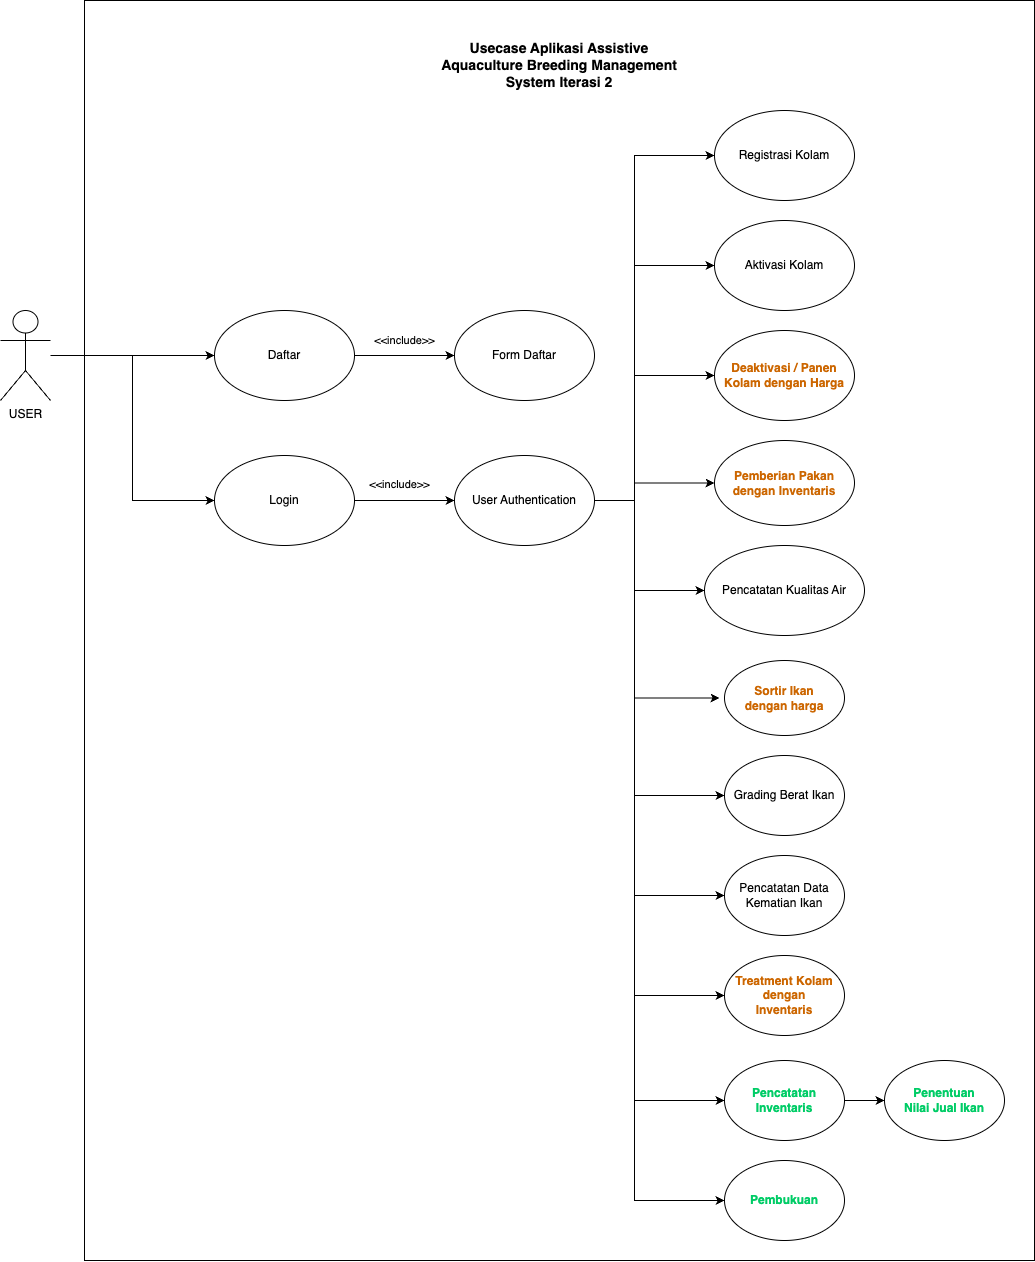
\includegraphics[width=1\textwidth]{gambar/usecase_iterasi_2.png}
	\caption{\textit{Use Case} Aplikasi}
\end{figure}

\section{Perancangan Sistem}

Pada aplikasi yang akan dibuat pada penelitian ini dikembangkan dengan metode Scrum. Beberapa komponen scrum seperti product backlog, sprint backlog, daily sprint, serta daily meet digunakan agar terwujudnya ketertiban dalam masa pengembangan aplikasi. Berikut penjelasan dari masing-masing elemen yang ada pada metode Scrum.

\begin{figure}[H]
	\centering
	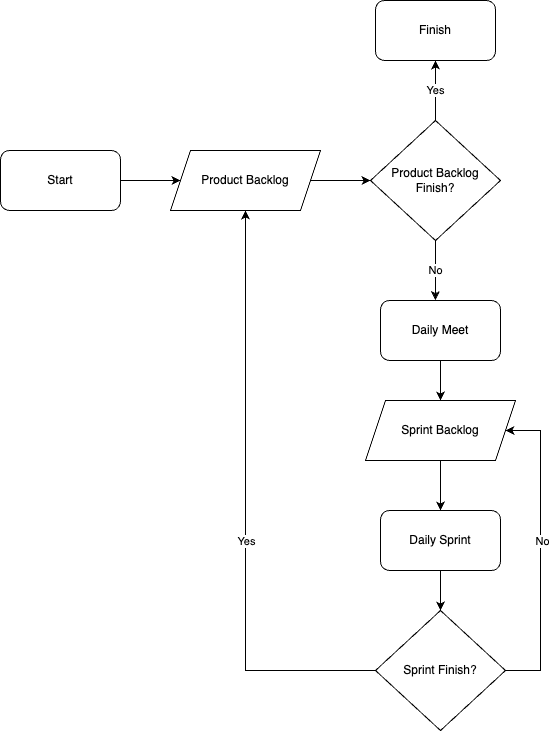
\includegraphics[width=0.8\textwidth]{gambar/scrum.png}
	\caption{Tahapan Perancangan Sistem dengan Metode Scrum}
\end{figure}

\begin{enumerate}
	\item Product Backlog
	
	Product Backlog adalah tugas-tugas yang \textbf{akan} dijalankan pada penelitian dan hal yang pertama kali dilakukan sebelum memulai riset. Daftar tugas yang ada pada Product Backlog ini akan dipindahkan pada Sprint Backlog tergantung pada skala prioritas dari task itu sendiiri. Berikut adalah tabel dari Product Backlog yang sudah berjalan.

	\begin{table}[H]	
		\begin{center}
			\caption{Product Backlog}
			\label{tab:table5}
			\begin{tabular}{|c|m{17em}|c|c|}
			\hline
			\textbf{No} & \textbf{Stories} & \textbf{Sprint} & \textbf{Status} \\
			\hline
			1 & Fitur Pencatatan inventaris & 1, 2, 3, 4, 5 & Selesai \\
			\hline
			2 & Fitur Aktivasi kolam dengan inventaris & 3, 4, 5 & Selesai \\
			\hline
			3 & Fitur Pemberian pakan yang terkoneksi dengan inventaris & 4 & Selesai \\
			\hline
			4 & Fitur Treatment kolam yang terkoneksi dengan inventaris & 5 & Selesai \\
			\hline
			5 & Fitur Panen termasuk harga nilai jual ikan & 5 & Selesai \\
			\hline
			6 & Fitur Pembukuan musim budidaya & 5 & Selesai \\
			% \hline
			% 7 & Fitur Depresiasi aset dalam inventaris & - & Tidak Selesai \\
			% \hline
			% 8 & Fitur Sortir termasuk harga nilai jual ikan & - & Tidak Selesai \\
			\hline
			\end{tabular}
		\end{center}
	\end{table}	

	\item Sprint Backlog
	
	Sprint Backlog adalah daftar tugas yang \textbf{harus} dijalankan selama masa Sprint berlangsung. Tugas yang ada pada Sprint Backlog bersifat fleksibel seiring dengan berjalannya Sprint.

	\item Sprint
	
	Progres sprint dilaksanakan ketika list task pada sprint backlog sudah disepakati bersama. Periode pengerjaan sprint bervariasi tergantung pada kesulitan task dari sprint backlog tersebut.
	
	\item Sprint Review
	
	Setelah Sprint berjalan, setiap minggunya diadakan meet bersama tim untuk melaksanakan Sprint Review yang bertujuan untuk melaporkan perkembangan Sprint baik itu proses ataupun hambatan selama pengerjaan Sprint.
	
	\hfill \break

	\item Deploy Sistem
	
	Ketika semua task sprint yang ada di sprint backlog selesai, maka aplikasi akan di deploy untuk dijalankan pengujian pada aplikasi. Pengujian aplikasi ini dilakukan dengan menggunakan Unit Testing dan User Acceptance Test (UAT).
	
\end{enumerate}

\section{Pengujian}

Di tahap pengujian ini, peneliti akan melakukan uji aplikasi menggunakan dua jenis pengujian yaitu unit testing dan UAT. Pengujian unit testing dilakukan oleh tim internal developer aplikasi untuk memastikan kepastian fungsi fitur dan cara kerja fitur agar aplikasi sesuai dengan kebutuhan. Sementara UAT dilakukan agar aplikasi dapat sesuai dengan kebutuhan \textit{user}.

\begin{enumerate}
	\item Unit Testing
	
	Pengujian dengan unit testing ini dibuat berdasarkan product backlog dan daftar sprint-sprint backlog yang sudah selesai. Berikut skenario pengujian yang akan dilakukan dapat dilihat pada \textbf{Tabel 3.2} berikut.

	\begin{table}[H]	
		\begin{center}
			\caption{Skenario Unit Testing}
			\label{tab:table8}
			\begin{tabular}{|m{13em}|m{17em}|}
			\hline
			\textbf{Jenis Fitur} & \textbf{Skenario Pengujian} \\
			\hline
			Fitur Pencatatan inventaris & Saat aplikasi dibuka, terdapat tombol Kolam yang ada di footer layar \\
			\hline
			 & Di halaman dashboard, terdapat tombol list yang ada pada pojok kiri atas aplikasi \\
			\hline
			 & Jika tombol list ditekan, maka akan tampil beberapa list menu inventaris \\
			\hline
			& Ketika salah satu tombol pada list inventaris ditekan, maka akan masuk ke halaman detail data inventaris dari menu yang dipilih \\
			\hline
			& Pada halaman detail data inventaris, ketika tombol riwayat di pojok kanan atas ditekan akan muncul rincian input pada sistem inventaris \\
			\hline
			& Pada halaman detail data inventaris, Ketika tombol (+) yang ada di pojok kanan bawah ditekan akan masuk ke halaman input data inventaris \\
			\hline
			Fitur Aktivasi kolam dengan inventaris & Pada halaman Aktivasi Kolam, terdapat list form yang harus diisi serta pilihan benih dari inventaris yang akan digunakan pada kolam tersebut.\\
			\hline
			\end{tabular}
		\end{center}
	\end{table}

	\begin{table}[H]	
		\begin{center}
			\begin{tabular}{|m{13em}|m{17em}|}
			\hline
			\textbf{Jenis Fitur} & \textbf{Skenario Pengujian} \\
			\hline	
			Fitur Pemberian pakan yang terkoneksi dengan inventaris & Pada halaman Rekap Data, terdapat tombol Rekapitulasi Pakan yang akan navigasi ke halaman Rekap Pakan \\
			\hline
			& Pada halaman Rekap Pakan, terdapat tombol Entry Pakan yang akan navigasi ke halaman Entry Pakan. Disini terdapat pilihan pakan yang sebelumnya sudah dimasukkan kedalam inventaris. \\
			\hline
			Fitur Treatment kolam yang terkoneksi dengan inventaris & Pada halaman Rekap Data, terdapat tombol Treatment yang ada pada header layar yang akan navigasi ke halaman Treatment. \\
			\hline
			& Pada halaman Treatment, terdapat tombol (+) yang ada dipojok kanan bawah layar yang akan navigasi ke halaman Input Treatment. \\
			\hline
			& Pada halaman Input Treatment, terdapat list form serta pilihan suplemen yang sebelumnya sudah dimasukkan ke dalam inventaris. \\
			\hline
			Fitur Panen termasuk harga nilai jual ikan & Pada halaman Panen, terdapat list form yang diisi untuk pendataan panen serta menunjukkan harga minimum ikan. \\
			\hline
			Fitur Pembukuan pencatatan pengeluaran permusim budidaya & Pada halaman Home, terdapat tombol buku di pojok kiri atas layar yang akan navigasi ke halaman Pembukuan. \\
			\hline
			& Pada halaman Pembukuan, terdapat list data ikan hasil panen dari tiap kolam. \\
			\hline
			\end{tabular}
		\end{center}
	\end{table}
	
	% \item User Analytics
	
	% Pengujian ini dilakukan kepada pembudidaya ikan dengan 3 tahap yaitu tutorial, logging / survei penggunaan aplikasi, dan interview. Tahapan tersebut dilakukan secara bertahap dan masing-masing tahap dijelaskan seperti berikut.

	% \begin{enumerate}
	% 	\item Tahap Tutorial
		
	% 	Pada tahap ini, dilakukan sesi pertemuan dengan para pembudidaya untuk menjelaskan fitur-fitur yang ada pada aplikasi secara keseluruhan.

	% 	\item Tahap Logging
		
	% 	Pada tahap ini, setiap aktivitas aplikasi yang dilakukan oleh pembudidaya akan dicatat oleh sistem. Hal ini mencakup seperti detail halaman yang diakses dan detail penggunaan fitur yang ada.
	
	% 	\item Tahap Interview
		
	% 	Pada tahap ini, terdapat sesi interview dengan pembudidaya mengenai penggunaan aplikasi. Dapat ditanyakan detail dari penggunaan aplikasi berdasarkan data logging yang sudah dikumpulkan sebelumnya.
	
	\item{\textit{User Acceptance Test}}

	User Acceptance Test dibuat berdasarkan fitur-fitur yang dapat diakses oleh pengguna pada product backlog. Berikut merupakan tabel format User Acceptance Test (UAT).

	\begin{longtable}[c]{@{} |p{1cm}|p{6.5cm}|p{1.1cm}|p{1.1cm}|p{1.1cm}|p{1.1cm}| @{}}
	\caption{Format \textit{User Acceptance Test} \label{uat}}\\

	\hline
	\multicolumn{6}{| c |}{\textbf{\textit{User Acceptance Test}}}\\
	\hline
	\multirow{2}{=}{\centering{\textbf{No}}} & \multirow{2}{=}{\centering{\textbf{\textit{Acceptance Requirements}}}} & \multicolumn{4}{| c |}{\textbf{Kesesuaian}}\\
	\cline{3-6}
	&  & \centering{\textbf{SS}} & \centering{\textbf{S}} & \centering{\textbf{TS}} & \centering{\textbf{STS}}
	\endfirsthead

	\hline
	\multicolumn{6}{| c |}{\textbf{\textit{User Acceptance Test}}}\\
	\hline
	\multirow{2}{=}{\centering{\textbf{No}}} & \multirow{2}{=}{\centering{\textbf{\textit{Acceptance Requirements}}}} & \multicolumn{4}{| c |}{\textbf{Kesesuaian}}\\
	\cline{3-6}
	&  & \centering{\textbf{SS}} & \centering{\textbf{S}} & \centering{\textbf{TS}} & \centering{\textbf{STS}}
	\endhead

	\hline
	\endfoot

	\hline
	\endlastfoot

	\hline
	1 & Fitur inventaris pakan &  &  &  &\\
	\hline
	2 & Fitur inventaris suplemen &  &  &  &\\
	\hline
	3 &	Fitur inventaris benih &  &  &  &\\
	\hline
	4 & Fitur inventaris listrik &  &  &  &\\
	\hline
	5 & Fitur inventaris aset &  &  &  &\\
	\hline
	6 & Aktivasi kolam dengan inventaris &  &  &  &\\
	\hline
	7 & Pemberian pakan dengan inventaris &  &  &  &\\
	\hline
	8 & Treatment kolam dengan inventaris &  &  &  &\\
	\hline
	9 & Panen kolam dengan harga jual minimum ikan &  &  &  &\\
	\hline
	10 & Pembukuan panen musim budidaya &  &  &  &\\
	\hline
	\end{longtable}
\end{enumerate}

% \subsection*{Daily Scrum}

% Daily Scrum merupakan kegiatan rutin tiap minggu yang dilaksanakan dengan Scrum Master. Kegiatan ini dilakukan untuk reporting progres tugas yang dijalankan selama masa Sprint berlangsung kepada Scrum Master. Scrum Master bertugas untuk memberikan feedback saat Daily Scrum berlangsung.

% \subsection*{Sprint Review dan Sprint Restropective}

% Sprint Review dan Sprint Restropective adalah kegiatan mengulas kembali tugas yang sudah dikerjakan pada saat durasi Sprint berlangsung. Kegiatan ini juga merupakan kegiatan menentukan tugas yang berhasil dan tidak berhasil selama Sprint berlangsung

\end{spacing}
